\documentclass{article}
\usepackage{hyperref}
\usepackage{graphicx}
\usepackage{listings}
% \documentclass[12pt,a4paper]{article}
% \usepackage{graphicx}

\title{INFO-F-311: Artificial Intelligence - Project 1: Search}
\author{Your Name}
\date{}

\begin{document}

\maketitle

\section{Preamble}
This report outlines the implementation of artificial intelligence techniques 
based on graph search techniques like 
Breadth-First Search (BFS), Depth-First Search (DFS), and the A* algorithm. 

The primary languages and tools used are Python 3.10 and Poetry.

\subsection{The Problems}
\begin{enumerate}
    \item \textbf{SimpleSearchProblem}: The goal is to reach the exit of the environment with multiple agents.
    \item \textbf{CornerSearchProblem}: The agents must pass through all four corners of the environment before reaching an exit.
    \item \textbf{GemSearchProblem}: The agents need to collect all gems in the environment before reaching an exit.
\end{enumerate}

\section{SimpleSearchProblem}

\subsection{Problem Modeling}
This section describes the is\_goal\_state and get\_successors methods.

\subsection{Breadth-First Search}
The Breadth-First Search algorithm is implemented in \texttt{search.py} via the \texttt{bfs} function.

\subsection{Depth-First Search}
The Depth-First Search algorithm is implemented in \texttt{search.py} via the \texttt{dfs} function.

\subsection{A* Search}
The A* algorithm is implemented with Manhattan distance as the heuristic.

\section{CornerSearchProblem}

\subsection{Problem Modeling}
The problem aims to pass through all four corners of the grid.

\subsection{Heuristic}
A consistent heuristic more efficient than Manhattan distance is developed.

\section{GemSearchProblem}

\subsection{Problem Modeling}
The problem aims to collect all gems in the environment.

\subsection{Heuristic}
A consistent heuristic more efficient than Manhattan distance is developed.


\section{Understanding the Code}

The codebase includes utility functions for calculating distances, an abstract SearchProblem class, and concrete problem classes like SimpleSearchProblem, CornerSearchProblem, and GemSearchProblem.

\subsection{Key Methods}
\begin{itemize}
    \item \texttt{is\_goal\_state()}: Determines if a state is the goal state.
    \item \texttt{get\_successors()}: Generates possible successor states from the current state.
    \item \texttt{heuristic()}: Calculates the heuristic value for the A* algorithm.
\end{itemize}


\section{Results}
\subsection{Path Size Comparison}
Comparison of the path sizes found by BFS, DFS, and A* on level 3.

\subsection{Node Expansion Comparison}
Comparison of the number of nodes expanded in BFS, DSF, and A* during the solution of level 3.

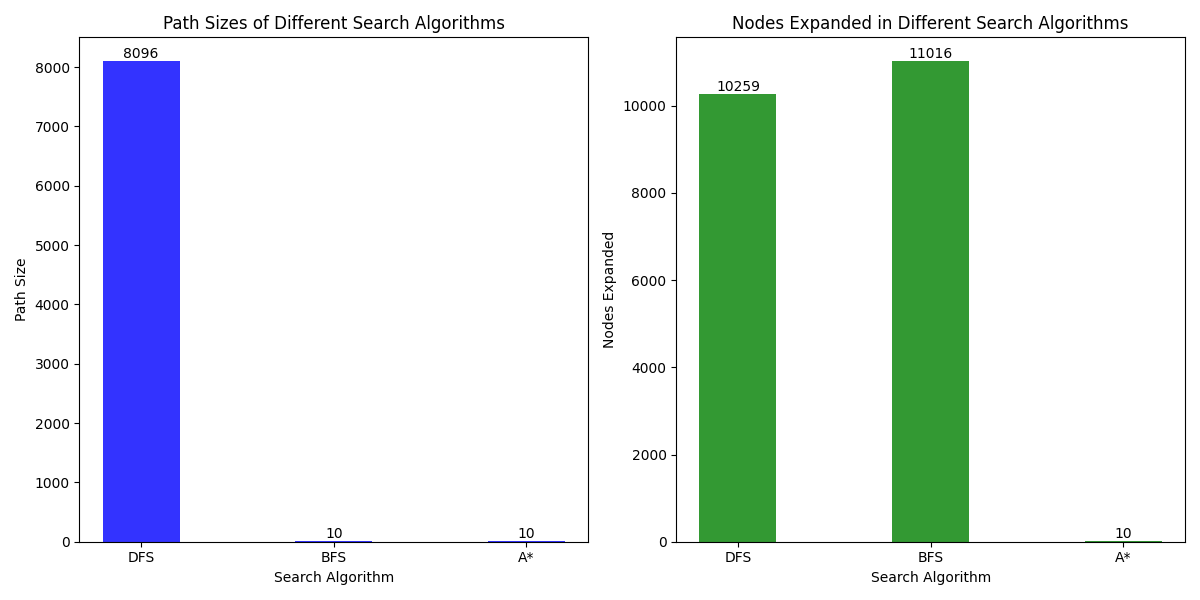
\includegraphics[width=\textwidth]{media/Figure_1.png}


\begin{tabular}{|c|c|c|c|}
    \hline
    Algorithm & Path Size & Nodes Expanded \\
    \hline
    DFS & 8096 & 10259 \\
    BFS & 10 & 11016 \\
    A* & 10 & 10 \\
    \hline
\end{tabular}

\subsection{Discussion}
\begin{itemize}
    \item \textbf{Efficiency}: A* is the most efficient in terms of both path size and nodes expanded.
    \item \textbf{Optimality}: BFS and A* find the optimal path, while DFS does not.
    \item \textbf{Resource Usage}: DFS and BFS are resource-intensive, whereas A* is memory-efficient.
    \item \textbf{Applicability}: A* is often the best choice when an admissible heuristic is available.
    \item \textbf{Path Quality}: DFS finds a path but not necessarily the shortest one.
    \item \textbf{Deterministic Outcome}: A* and BFS provide a more predictable and optimal outcome compared to DFS.
\end{itemize}    



\section{Heuristics Development}
    heuristic for CornerSearchProblem and GemSearchProblem.

\section{Optimizations}
\begin{itemize}
    \item Use a priority queue for the A* algorithm.
    \item Cache heuristic values to avoid redundant calculations.
\end{itemize}

\section{Tool Usage}
Explanation of the use of tools like ChatGPT in the project.

\subsection{Initial Phase: Data Dump}
In the initial stage, I fed ChatGPT with as much contextual information as possible. 
\begin{itemize}
    \item INFO-F-311_ Project1
    \item 1-recherche-v3.zip
    \item Project challenges
    \item Project resources
    \item Project timeline

This process is analogous to brainstorming with another person but in a more structured and data-driven manner.

\subsubsection{Memory}

Each time new 

\subsection{Fine-Tuning Perception}
After the initial data input, I fine-tuned how ChatGPT interprets the provided information. 
This involved adjusting the focus towards specific problem statements and goals. 
The objective was to align the AI's understanding with the project requirements.

\subsection{Filtering Output}
ChatGPT's output also underwent a filtration process to distill the most useful and relevant suggestions or solutions. 
This step ensured that the AI's contributions were directly applicable to the project.

\subsection{Comparative Analysis}
While ChatGPT was processing data and generating insights, I also developed my own ideas and solutions. This dual approach allowed for a comprehensive comparative analysis, which often led to more refined and effective strategies for tackling the project's challenges.

\subsection{Synergistic Collaboration}
The combination of human intuition and AI-generated insights created a synergy that enriched the project's development process. It was like having an extra team member who could offer a different perspective, thereby broadening the scope and enhancing the quality of the project.

\subsection{Advantages \& Limitations}
The primary advantage of using ChatGPT was the acceleration of the ideation and problem-solving phases. However, it's essential to note that while the tool provided rapid insights, the quality and applicability of these insights still required human judgment for effective implementation.


\end{document}
